\documentclass[a4paper,12pt,ngerman,fleqn]{article}

    \renewcommand{\familydefault}{\sfdefault}
    \usepackage[a4paper, margin={0cm,0cm},twocolumn, layouthoffset=0pt]{geometry}
    
    \usepackage{tikz}
    \usepackage{framed}
    \usepackage{amsmath}
    \setlength{\mathindent}{0pt}
    \usepackage{amsfonts}
    \usepackage{amssymb}
    \usepackage{tabularx, colortbl}

    \usepackage{xcolor}
    \definecolor{accent}{HTML}{0eb7ac}

    \linespread{1}
    \vspace{1cm}
    \renewcommand{\arraystretch}{2}
    \arrayrulecolor{accent}
    \setlength\arrayrulewidth{1.5pt}
    \renewcommand{\baselinestretch}{0.8} 
    \newcommand{\mybox}[3]{
        \centering
        \begin{tabularx}{0.9\textwidth}{|X|}
            \rowcolor{accent}
            \rule{0pt}{20pt}
            \textcolor{white}{\textbf{#1}} \\
            \def\temp{#2}\ifx\temp\empty
                
            \else
                #2 \\ \hline
            \fi
            #3
            \\ \hline
        \end{tabularx}
    }

\begin{document}
    
    \setlength{\parindent}{0cm}

    \begin{tikzpicture} 
        \fill[accent, opacity=1] (0,0) rectangle (21,3);
        \fill[accent, opacity=0.8] (0,-2) rectangle (21,0);
        \fill[accent, opacity=1] (1.5,0.1)
            -- (2,-0.5)
            -- (2.5,0.1)
            -- cycle;
        \node[anchor=east,text=white] (why1) at (7.6,1.5) {\huge Logistic Regression};
        \node[anchor=east,text=white] (why1) at (14.7,-0.9) {
            Logistic Regression: is named that way for historical reasons and is actually an
        };
        \node[anchor=east,text=white] (why1) at (11.6,-1.4) {
            approach to classification problems, not regression problems.
        };
    \end{tikzpicture}

    % LEFT SIDE OF SHEAT
    \begin{minipage}[t]{.51\textwidth}
        \vspace{1pt}
        \mybox
            {Binary Classification - Sigmoid}
            {
                \rule{0pt}{20pt}
                \( g(z) = \dfrac{1}{1 + e^{-z}} \) \\
                {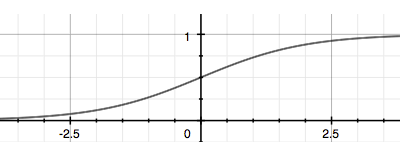
\includegraphics[width=0.85\textwidth, height=40mm]{sigmoid.png}}
            }
            {
                hypothesis should satisfy: \( 0 \leq h_\theta(x) \leq 1 \)
            }
        \newline
        \newline
        \newline
        \mybox
            {Decision Boundary}
            {
                \( h_\theta(x) \geq 0.5 \rightarrow y = 1 \) \\
                \( h_\theta(x) < 0.5 \rightarrow y = 1 \)
            }
            {
                translate the output of the hypothesis function
            }
        \newline
        \newline
        \newline
        \mybox
            {Cost Function}
            {
                \rule{0pt}{20pt}
                \( J(\Theta) = \dfrac{1}{m} \sum\limits_{i=1}^{m}(Cost(h_\theta(x_{(i)}), y_{(i)})) \) \\
                \(\mathrm{Cost}(h_\theta(x),y) = -\log(h_\theta(x)) \) if y = 1 \\
                \(\mathrm{Cost}(h_\theta(x),y) = -\log(1-h_\theta(x)) \) if y = 0
            }
            {
                {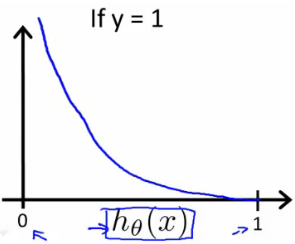
\includegraphics[width=0.4\textwidth, height=35mm]{y=1.png}}
                {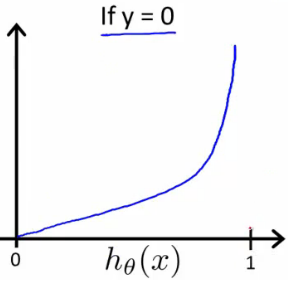
\includegraphics[width=0.4\textwidth, height=35mm]{y=0.png}}\\ \hline
                \(\mathrm{Cost}(h_\theta(x),y) = 0 \text{  if  } h_\theta(x) = y \) \\
                \(\mathrm{Cost}(h_\theta(x),y) \rightarrow \infty \text{  if  } y = 0 \mathrm{and} h_\theta(x) \rightarrow 1 \) \\
                \(\mathrm{Cost}(h_\theta(x),y) \rightarrow \infty \text{  if  } y = 1 \mathrm{and} h_\theta(x) \rightarrow 0 \)
            }
        \newline
    \end{minipage}%
    \begin{minipage}[t]{.51\textwidth}
        \vspace{1pt}
        \mybox
            {Gradient Descent}
            {}
            {
                \( Repeat \; \lbrace \) \\
                \( \theta_j := \theta_j - \frac{\alpha}{m} \sum_{i=1}^m (h_\theta(x^{(i)}) - y^{(i)}) x_j^{(i)} \) \\
                \(\rbrace\)
            }
        \newline
        \newline
        \newline
        \mybox
            {Simpliefied Cost Function}
            {}
            {
                \( J(\Theta) = \dfrac{1}{m} \sum\limits_{i=1}^{m}[y^{(i)}log(h_\theta(x^{(i)})) + \) \\
                \rule{38pt}{0pt}
                \( (1 - y^{(i)})log(1 - h_\theta(x^{(i)}))] \)
            }
        \newline
    \end{minipage}

    \vspace{54.5pt}
    \fcolorbox{accent}{accent}{
    \begin{minipage}[t]{1\textwidth}
        \vspace{2pt}
        \center
        \textcolor{white}{\scriptsize \copyright 2018 - Hacky footer }
        \vspace{2pt}
    \end{minipage}
    }
    
\end{document}